\chapter*{decay}
\addcontentsline{toc}{chapter}{decay}
\begin{center}
\vspace{2cm}
\begin{flushright}
\large
\textit{ $n \rightarrow p^+ + e^- + \bar{\nu}_e$ }
\end{flushright}
\vspace{2cm}
% \vspace*{\fill}
\end{center}
\normalsize

\newpage  % Move to the next page
Decay is a fundamental process of transformation, marking the passage from one state of existence to another. In physics, decay symbolizes change, entropy, and the relentless flow of time. When an atom has an unstable configuration, such as an excess of neutrons, it undergoes decay to achieve stability. A neutron transforms into a proton, emitting an electron and an antineutrino in the process, in a phenomenon known as beta-minus decay.

%% image
\begin{figure}
    \centering
    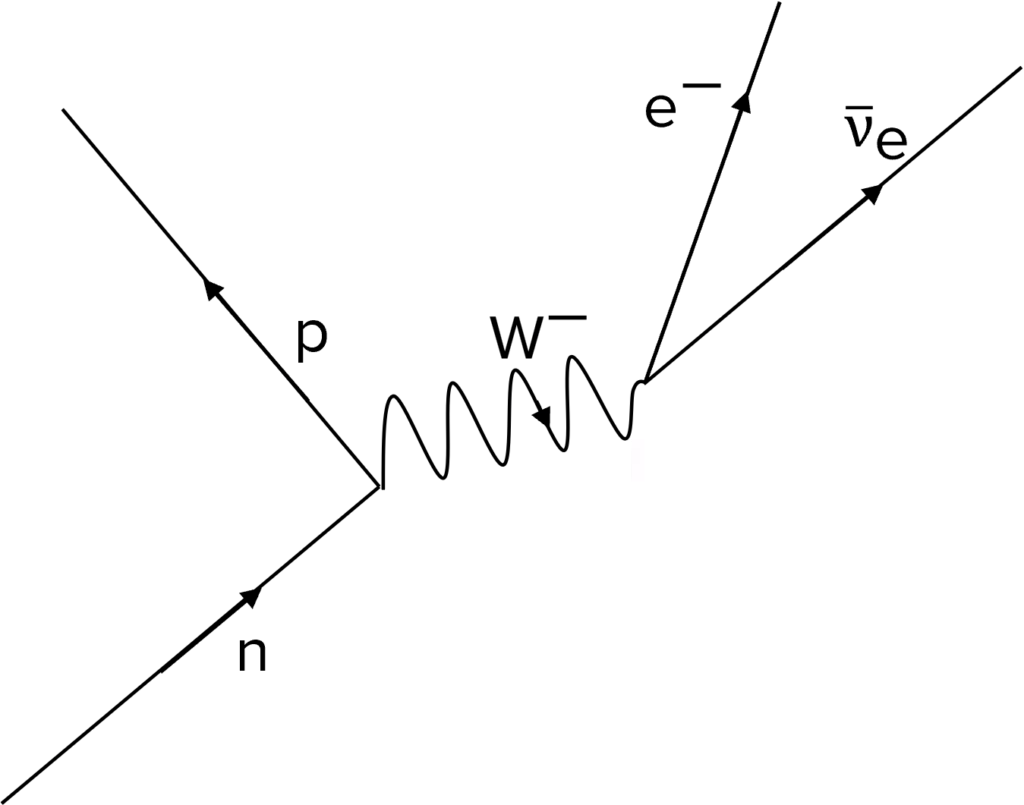
\includegraphics[width=0.8\linewidth]{assets/betaminusdecay.png} 
    \caption{\small Beta-minus decay.}
    \label{fig:betaminusdecay}
\end{figure}

Just as the carbon-14 that undergoes radioactive decay over millennia, serving as a measure of time and history, our lives too are governed by the forces of transformation and impermanence. The weight of indecision, uncertainty, and imbalance manifests as forces propelling us toward change. And like nitrogen-14, the stable product of decay, we seek equilibrium, a resolution to the chaos that defines our existence. Much like the emitted radiation in atomic decay, the disruptions and losses we experience are the byproducts of our transformation.

In the digital realm, decay mirrors the entropic nature of information and memory. Glitches, data loss, and the degradation of digital media are reminders of the fragility of permanence in a system that relies on energy and maintenance. Artists and technologists alike have explored the concept of digital decay, creating dynamic pieces designed to purposefully degrade and transform over time. These works challenge the idea of art as a static entity, taking advantage of the beauty of impermanence.

Everything is transient, every present moment unfolds from the past. Processes of becoming and unbecoming underscore the interconnectedness of all phenomena. Decay drives the universe toward higher entropy, as described by the second law of thermodynamics, defining the arrow of time. Entropy is not merely a measure of chaos but a sign of the potential for transformation. Decay is a precondition for creation.

% note: glitch ?

% Dieter Roth - biodegradable artworks - https://www.tate.org.uk/art/artists/dieter-roth-1870

% The Disintegration Loops is a series of four albums by the American avant-garde composer William Basinski,
% https://en.wikipedia.org/wiki/The_Disintegration_Loops

% note : use this example... dementia ---
% Everywhere at the End of Time[a] (commonly shortened to EATEOT) is the eleventh recording by the Caretaker, an alias of English electronic musician Leyland Kirby. Released between 2016 and 2019, its six studio albums use degrading loops of sampled ballroom music to portray the progression of dementia and related neurological conditions
% Decay serves as both an end and a beginning. It is the dissolution of what was and the emergence of what could be. In embracing decay, we accept the inevitability of change and the transformative power it holds. Whether in the disintegration of memory or the breakdown of stability, decay serves as an excuse to find value and meaning in impermanence.


% note: art or culture for that matter represent 'negentropy': an effort to fight against the tendency of collapse .
